\documentclass[NET,english,beameralt,aspectratio=169]{tumbeamer}

% If you load additional packages, do so in packages.sty as figures are build
% as standalone documents and you may want to have effect on them, too.

% Folder structure:
% .
% ├── beamermods.sty                  % depricated an will be removed soon
% ├── compile                         % remotely compile slides
% ├── figures                         % all figures go here
% │   └── schichtenmodelle_osi.tikz   % each .tikz or .tex is a target
% ├── include                         % create your document here
% │   ├── example.tex                 % example document
% │   └── slides.tex                  % make document wide changes here
% ├── lit.bib                         % literature
% ├── Makefile
% ├── moeptikz.sty                    % fancy networking symbols
% ├── packages.sty                    % load additional packages there
% ├── pics                            % binary pcitures go here
% ├── slides.tex                      % main document (may be more than one)
% ├── tumbeamer.cls
% ├── tumcolor.sty                    % TUM color definitions
% ├── tumcontact.sty                  % TUM headers and footers
% ├── tumlang.sty                     % TUM names and language settings
% └── tumlogo.sty                     % TUM logos

% Configure author, title, etc. here:
\usepackage[utf8]{inputenc}
\usepackage{packages}
\usepackage{beamermods}

%do not load enumitem with beamer


%stand alone entries for my own pubs
%http://stefaanlippens.net/bibentry/
%\usepackage{natbib}
\usepackage{bibentry}
\nobibliography*

% For beamer mode (default):
\author[C.\ Diekmann]{Cornelius Diekmann, M.\,Sc.}
\title[Provably Secure Networks: Methodology and Toolset for Configuration Management]{Provably Secure Networks:\\Methodology and Toolset for Configuration Management}
\date{July 27, 2017}

\usepackage{pgfpages}
\usepackage{ifthen}


%\setbeameroption{show notes on second screen=right}


\newcommand{\hairspace}{\hspace{1pt}}
\newcommand{\eg}{\mbox{e.\hairspace{}g.,} }  % z.B.
\newcommand{\ie}{\mbox{i.\hairspace{}e.,} }  % d.h.
\newcommand{\Ie}{\mbox{I.\hairspace{}e.,} }  % d.h.
\newcommand{\cf}{\mbox{cf.}\ }
\newcommand{\etal}{\mbox{et~al.}\ }

\usepackage{fancyvrb}

\usepackage{IEEEtrantools}

%https://tex.stackexchange.com/questions/220820/itemize-list-inside-a-tikzpicture-node
\usepackage{varwidth}

% math typesetting
% free variables
\newcommand{\mvar}[1]{\ensuremath{\mathit{#1}}}
% definitions and constants
\newcommand{\mdef}[1]{\ensuremath{\mathsf{#1}}}
% executable functions
\newcommand{\mfun}[1]{\mdef{#1}}
%datatype constructor (may appear in text)
\newcommand\mconstr[1]{\mdef{#1}}
%math control (if then else)
\newcommand\mctrl[1]{\ensuremath{\mathbf{#1}}}


\newcommand{\topos}{\emph{topoS}}
\newcommand{\fffuu}{\emph{{f}{f}{f}uu}}

\newcommand\iptables{{iptables}}


\newcommand{\BigO}{\mathcal{O}}


\DeclareMathSymbol{\mlq}{\mathord}{operators}{``}
\DeclareMathSymbol{\mrq}{\mathord}{operators}{`'}


\newcommand\mdoubleplus{\ensuremath{\mathbin{+\mkern-10mu+}}}
\newcommand\lstapp{\ensuremath{\mathbin{:\mkern-1mu:\mkern-1mu:}}} %list append
\newcommand\lstcons{\ensuremath{\mathbin{:\mkern-1mu:}}} %list append

\newcommand{\free}[1]{\textcolor{TUMDarkerBlue}{#1}}
\newcommand{\bound}[1]{\textcolor{TUMDarkGreen}{#1}}
\newcommand{\boundi}[1]{\textcolor{TUMGreen}{#1}}


\newcommand*\circled[1]{\tikz[baseline=-3pt, scale=0.5, every node/.style={scale=0.5}]{\node[shape=circle,draw,inner sep=1pt,minimum size=16pt] (char) {#1};}}

\newcommand\allow{\ensuremath{\textnormal{\circled{\large \textbf{\checkmark}}}}}
\newcommand\deny{\ensuremath{\textnormal{\circled{\large \textbf{\texttimes}}}}}
\newcommand\undecided{\ensuremath{\textnormal{\circled{\textnormal{\large \textbf{?}}}}}}

\newcommand\matchop[1]{\ensuremath{\mfun{match}\ {#1}}}
\newcommand\matches[1]{\ensuremath{\matchop\gamma \ #1 \ p}}
\newcommand\nmatches[1]{\ensuremath{\neg\; \matchop\gamma \ #1 \ p}}
\newcommand\bigstep[3]{\ensuremath{\free{\Gamma},\free{\gamma},\free{p} \vdash\big\langle #1,\; #2 \big\rangle \Rightarrow #3}}

%https://tex.stackexchange.com/questions/85284/pointing-an-arrow-to-a-tabular-node-in-beamer-is-buggy-ignorenonframetext
\tikzset{every picture/.style={remember picture}}



%http://tex.stackexchange.com/questions/84143/fancy-arrows-with-tikz
\tikzset{MyDoubleArrow/.style={double arrow, draw=black, anchor=west, align=center, text width=2em}}
\tikzset{MySingleArrow/.style={single arrow, draw=black, anchor=west, align=center, text width=2em}}
\tikzset{MySingleLeftArrow/.style={single arrow, rotate=180, draw=black, anchor=east, align=center, text width=2em}}

\tikzset{MyRoundedBox/.style={
		draw,
		rounded corners=3pt,
		inner sep=3pt,
		anchor=west,
		text width=11em,
		%minimum height=8ex,
		align=center,
		fill=TUMYellow,
	}
}


\usetikzlibrary{arrows.meta} %requires pgf > 3.0.

\tikzset{myptr/.style={-{Latex[scale=1.5]}}}%
\tikzset{myptrdouble/.style={{Latex[scale=1.5]}-{Latex[scale=1.5]}}}%
\tikzset{myptrdotted/.style={myptr,dashed}}%

\newcommand{\blitzbam}{
\includegraphics[height=4em]{pics/blitz.pdf}}


\begin{document}

% If you are preparing a talk but do not like the default font sizes, you may
% want to try the class option 'beameralt', which uses smaller default font
% sizes and integrates subsection/subsubsection names into the headline.

% For lecture mode, you may want to build one set of slides per chapter but
% with common page numbering. If so,
% 1) create a new .tex file for each chapter, e.g. slides_chapN.tex,
% 2) set the part counter to N-1 (assuming chapters start at 0), and
% 3) and name your chapter by using the \part{} command.
%\setcounter{part}{-1}
%\part{Organisatorisches und Einleitung}

% For 16:9 slides, use the class option 'aspectratio=169'.

% If class option 'noframenumbers' is given, frame numbers are not printed.

% If class option 'notitleframe' is given, the title frame is not autmatically
% generated.

% Class option 'nocontentframes' suppresses automatic generation of content
% frames when new parts/sections are started.

% Include source files from ./include (or ./include/chapN).
\section{Motivational Quote}
\begin{frame}
	%\begin{Large}
	\begin{center}
    \onslide<1->{``\textit{there are no good high-complexity rule sets}''\\\hspace*{15em}{\small--- A.\ Wool, 2004}}\bigskip\\
	\onslide<2->{``\textit{firewalls are (still) poorly configured}''\\\hspace*{15em}{\small--- A.\ Wool, 2010}}\bigskip\\
	\onslide<3->{\dots}\bigskip\\
	\note<3->[item]{Current papers also regularly report this issue. Our findings underline this.}
	%\onslide<3->{``\textit{tools do not understand real-world firewall rules}''} [Diekmann 2015]\bigskip\\
	\end{center}
	%\end{Large}
\end{frame}

\section{Research Question}
\begin{frame}
	\begin{large}
	\begin{center}
	How can we help administrators to configure secure networks\\and\\ verify the security of existing network configurations?
	\end{center}
	\end{large}
	\note[item]{Network access control}
	\note[item]{Configuration (of e.g.\ firewall)}
	\note[item]{Administration}
	\note[item]{Security}
\end{frame}

\section{Agenda}
\begin{frame}
	\begin{enumerate}
		\addtolength{\itemsep}{3ex}
		\item My Contributions \& My Thesis
		\note[item]{Time constraints, only an overview}
		\item Selected Topic: Case Study
		\note[item]{One chapter (one of my favorite), example story, demonstrate all the results}
		\item State-of-the-Art \& Related Work
		\note[item]{Others tries to tackle these problems before}
	\end{enumerate}
\end{frame}


\section{Structured Approach: Security Components}
\begin{frame}
	\note[item]{No talking about `security' without defining \emph{secure} and what can go wrong.}
	Inspired by Bishop [S\&P vol.\ 1, 2003] and taught in ``Network Security'' at TUM.\vspace*{10ex}
	%\footnote{M. Bishop, \textit{``What Is Computer Security?''} IEEE Security \& Privacy, vol.\ 1, no.\ 1, Feb.\ 2003.}
	%\cite{bishop2003compsec}
	 \begin{center}
	    %\resizebox{0.99\textwidth}{!}
	 \end{center}
	\begin{tikzpicture}[overlay]
		\node<2>[anchor=north west] (sinvarlabel) at ($(sinvar.west)+(0em,-5em)$) {Scenario-specific security goals (high level of abstraction)};
	    \path[myptr]<2> (sinvarlabel) edge (sinvar);
	    
		\node<3>[anchor=north] (policylabel) at ($(policy)+(0em,-5em)$) {\textbf{Enforceable} rules};
	    \path[myptr]<3> (policylabel) edge (policy);
	    
		\node<4>[anchor=north east] (mechanismlabel) at ($(mechanism.east)+(0em,-5em)$) {Firewall Rules, OpenFlow Tables, \dots (low-level details)};
	    \path[myptr]<4> (mechanismlabel) edge (mechanism);
	    \note<4>{Disregarding hardware rootkits, security holes in mechanism itself. Firewalls pretty robust (most, \dots)}
	    
	    \note<5->{Security problems.}
	    \node<6> at ($(sinvar) + (0ex,0ex)$) {\blitzbam};
	    
	    \node<7> at ($(arr1) + (0ex,0ex)$) {\blitzbam};
	    \node<7> at ($(arr2) + (0ex,0ex)$) {\blitzbam};
	    
	    \node<8> at ($(mechanism) + (0ex,0ex)$) {\blitzbam};
	\end{tikzpicture}
	
	\onslide<5->{
	Security Problems
	\begin{itemize}
		\item<6-> Unsuitable requirements
			\note<6>[item]{No requirements specification; Requirements do not mean what they should}
		\item<7-> Translation error
			\note<7>[item]{policy does not enforce requirements}
			\note<7>[item]{low-level: shadowed firewall rules}
		\item<8-> Bug in the mechanism (not part of this thesis)
			\note<8>[item]{Bugs in firewall software relatively rare -- compared to bad policies}
	\end{itemize}
	}
\end{frame}





\section{Contents of My Thesis}

\begin{frame}[t]
  \begin{center}
  %\resizebox{0.99\textwidth}{!}{%
  \begin{tikzpicture}
  \node [MyRoundedBox](sinvar) at (0,0) {\strut{}Security Requirements};
  \node [MyDoubleArrow](arr1) at (sinvar.east) {};
  \node [MyRoundedBox](policy) at (arr1.east) {\strut{}Security Policies};
  \node [MyDoubleArrow](arr2) at (policy.east) {};
  \node [MyRoundedBox](mechanism) at (arr2.east) {\strut{}\only<1-4>{Security Mechanisms}\only<5->{\texttt{iptables}}};
  
  \visible<2-6>{\node[anchor=north] at ($(sinvar) + (0,-1em)$) {Part~1};}
  \visible<5-6>{\node[anchor=north] at ($(mechanism) + (0,-1em)$) {Part~2};}
  
  \draw<3-6>[shorten <=-2cm,shorten >=-1ex,myptr] ($(arr1) + (0,3em)$)--($(policy) + (0,3em)$);
  \visible<3-6>{\node[anchor=south] at ($(arr1) + (0,3em)$) {Part~1};}
  \draw<4-6>[shorten <=2ex,shorten >=-2cm,myptr] ($(policy) + (0,3em)$)--($(arr2) + (0,3em)$);
  \visible<4-6>{\node[anchor=south] at ($(arr2) + (0,3em)$) {Part~1};}
  \draw<6-6>[shorten <=-2cm,shorten >=-1ex,myptr] ($(arr2) + (0,-3em)$)--($(policy) + (0,-3em)$);
  \visible<6-6>{\node[anchor=north] at ($(arr2) - (0,3em)$) {Part~2};}
  %\draw<6-6>[shorten <=2ex,shorten >=-2cm,dashed,myptr] ($(policy) + (0,-3em)$)--($(arr1) + (0,-3em)$);
  %\visible<6-6>{\node[anchor=north] at ($(arr1) - (0,3em)$) {Part~2};}
  
  \visible<7->{\path[draw,myptr,shorten >=0.5cm,shorten <=0.5cm] 
  (sinvar) to[bend left]    node[anchor=south, yshift=1ex] {\topos{} Policy Construction} (policy);}

  \visible<7->{\path[draw,myptr,shorten >=0.5cm,shorten <=0.5cm] 
  (policy) to[bend left]    node[anchor=south, yshift=1ex] {\topos{} Serialize} (mechanism);}

  \visible<7->{\path[draw,myptr,shorten >=0.5cm,shorten <=0.5cm] 
  (mechanism) to[bend left]    node[anchor=north, yshift=-1ex] {\fffuu{} Service Matrices} (policy);}

  \visible<7->{\path[draw,dashed,myptr,shorten >=0.5cm,shorten <=0.5cm] 
  (policy) to[bend left]    node[anchor=north, yshift=-1ex] {\topos{} Verification} (sinvar);}
  \end{tikzpicture}%
  %}
  \end{center}
  \begin{columns}[t]
	\begin{column}{0.35\textwidth}
		\only<2-4>{Part~1
	  	\begin{itemize}
	  		\item<2-> Specifying security requirements
	  			\begin{itemize}
	  			\item Chapters 5, 6
	  			\end{itemize}
	  		\item<3-> Translating to an enforceable policy
	  			\begin{itemize}
	  			\item Chapters 7, 8, 9
	  			\end{itemize}
	  		\item<4-> Deploying to devices
	  			\begin{itemize}
	  			\item Chapter 10
	  			\end{itemize}
	  			\note{Discussing assumptions of theory, ...}
	  	\end{itemize}%
	  	}%
	  	\only<5-6>{Part~2
	  	\only<5>{\addtocounter{framenumber}{1}} %new slide
	  	\begin{itemize}
	  		\item<5-> Focus on \texttt{iptables}
	  			\begin{itemize}
	  			\item Chapters 12, 13
	  			\end{itemize}
	  			\note<5->{Formal semantics in 12, spoofing in 13}
	  		\item<6-> Inferring policy from low-level rules
	  			\begin{itemize}
	  			\item Chapter 14
	  			\end{itemize}
	  			\note<6->{Low-level details such as IP address spoofing. Analyzing existing installations. }
	  	\end{itemize}%
	  	}%
	  	\only<7->{Part~3
	  	\only<7>{\addtocounter{framenumber}{1}} % new slide
	  	\begin{itemize}
	  		\item Demonstrate applicability
	  			\begin{itemize}
	  			\item Chapter 16: Docker \onslide<8->{\emph{$\longleftarrow$ next}}
	  			\item Chapter 17: MeasrDroid
	  			\end{itemize}
	  			\note<8->{limited time}
	  		\item Summary of scientific results, comparison to state-of-the-art
	  			\begin{itemize}
	  			\item Chapters 18, 19, 20, 21
	  			\end{itemize}
		\end{itemize}
		}
	\end{column}
	\begin{column}{0.60\textwidth}
		\only<2>{%Part~1
	  	\begin{itemize}
	  		\item Security Invariants
	  			\begin{itemize}
	  			\item Generic part: template
	  			\item Generic proofs, \eg ``prohibiting more does not decrease security''
	  			\item Template library
	  			\item Scenario-specific part: user assigns attributes to hosts
	  			%\item Auto-completion with secure default values
	  			\end{itemize}
	  		\item Policy verification
	  	\end{itemize}
	  	}
		\only<3>{%Part~1
	  		\begin{itemize}
	  			%\item Automated
	  			\item Visual feedback
	  			\item Policy uniquely defined?
	  			\item Sound \& Complete
	  			\item Performance
	  			\item Connection level vs.\ network level and stateful flows
	  		\end{itemize}
	  	}
		\only<4>{%Part~1
	  		\begin{itemize}
	  			\item Discussing assumptions and implementation details
	  			\item Central \texttt{iptables} firewall, OpenVPN setup, OpenFlow
	  		\end{itemize}
	  		\note{Discussing assumptions of theory, ...}
	  	}%%%%
		\only<5>{%Part~2
	  	\begin{itemize}
	  		\item Formal semantics of \texttt{iptables}
	  		\begin{itemize}
	  			\item \emph{Arbitrary} match conditions
	  		\end{itemize}
	  		\item IPv4 \& IPv6
	  		\item Verify spoofing protection
	  		%\begin{itemize}
	  		%	\item Enables replacing matches on interfaces by matches on IP addresses
	  		%\end{itemize}
	  	\end{itemize}
	  	}%
		\only<6>{%Part~2
	  	\begin{itemize}
	  		%\item Automated
	  		\item Translate to a simplified firewall model
	  		\begin{itemize}
	  			\item Abstract over low-level details by overapproximation
	  		\end{itemize}
	  		\item Infer high-level policy
	  		\item If a firewall (probably) accepts a connection $\longrightarrow$\newline{} then the connection is (definitely) shown in our inferred policy
	  	\end{itemize}
	  	}%%%%
		\only<7->{%Part~3
	  	\begin{itemize}
	  		\item Further evaluation
	  		\begin{itemize}
  				\item Cabin data network
  				\item MeasrDroid privacy audit
  				\item Largest collection of public \texttt{iptables} dumps
	  		\end{itemize}
	  		\item Comparison to state-of-the-art \onslide<9->{\emph{$\longleftarrow$ This talk later}}
	  	\end{itemize}
	  	}
	\end{column}
	\end{columns}
\end{frame}

% it should take 10 minutes of talking to arrive here.


\section{Example: Specifying Security Requirements}
\begin{frame}

\setbeamercolor{alerted text}{fg=TUMOrange}

	\begin{minipage}{0.3\textwidth}\centering
	%\includegraphics[width=0.99\linewidth]{pics/net_schematic.pdf}
    \resizebox{0.99\textwidth}{!}{%
    \begin{Large}
    \begin{tikzpicture}
        %note, different coordinates (tighter packed) than images with ipaddresses
	   	\node[align=center,text width=8.5em,cloud, draw,cloud puffs=10,cloud puff arc=120, aspect=2, inner sep=-3em,outer sep=0] (inet) at (0,-.3) { \emph{INET} };
	   	\node[rectangle, fill=TUMLightGray] (networkbox) at (.6,-2) { \only<1>{Network}\only<2->{
\includegraphics[width=4em]{pics/docker.pdf}}};
	   	
	   	\node (webfrnt) at (3.8,-.6) { \emph{WebFrnt} };
	   	\node (webapp) at (2.5,-3.9) { \emph{WebApp} };
	   	\node (log) at (3.5,-3.4) { \emph{Log} };
	   	\node (db) at (4.3,-3.9) { \emph{DB} };

	    \draw (inet) node[label={[below,xshift=22,yshift=-13]Uplink}] {}--(networkbox);
	    \draw (networkbox)--(2,-1.2)node[label={[below,xshift=11,yshift=-2]DMZ}] {}--(5,-1.2);
	    \draw (networkbox)--(2,-2.8)node[label={[above,xshift=12,yshift=-4]Intern}] {}--(5,-2.8);
	    
	    \draw (3.8,-1.2)--(webfrnt);
	    \draw (2.5,-2.8)--(webapp);
	    \draw (3.5,-2.8)--(log);
	    \draw (4.3,-2.8)--(db);
    \end{tikzpicture}
    \end{Large}}
	\end{minipage}
	\hspace*{\fill}
	\begin{minipage}{0.5\textwidth}
		\begin{enumerate}
		\item \alert<3>{Logging data must not leave the \emph{Log} server.}

		\item \alert<4>{\emph{DB}, \emph{Log} and \emph{WebApp} are internal hosts. 
			\emph{WebFrnt} must be accessible from outside.} 

		\item \alert<5>{\emph{DB}, \emph{Log} contain confidential information. 
			\emph{Web\-App} is trusted and allowed to declassify.}

		\item \alert<6>{Only \emph{Web\-App} may access the \emph{DB}.}
		\end{enumerate}
	\end{minipage}
	\hspace*{\fill}

\bigskip

    \note{slightly simplified syntax for the talk.}
\visible<3->{
\fbox{
%\begin{mdframed}
\begin{minipage}{0.98\textwidth}
\begin{flushleft}
\smallskip
\visible<3->{\alert<3>{Sink $\lbrace \mathrm{\emph{Log}} \mapsto \mathit{Sink} \rbrace$}}

\medskip

\visible<4->{\alert<4>{SubnetsInGW $\lbrace \mathrm{\emph{DB}} \mapsto \mathit{internal},\ \mathrm{\emph{Log}} \mapsto \mathit{internal},\ 
\mathrm{\emph{WebApp}} \mapsto \mathit{internal},\ \mathrm{\emph{WebFrnt}} \mapsto \mathit{InboundGateway}
\rbrace$}}

\medskip

\visible<5->{\alert<5>{Bell LaPadula $\lbrace \mathrm{\emph{DB}} \mapsto \mathit{confidential},\ \mathrm{\emph{Log}} \mapsto \mathit{confidential},\ 
\mathrm{\emph{WebApp}} \mapsto \mathit{declassify} \ \mathit{(trusted)} \rbrace$}}

\medskip

\visible<6->{\alert<6>{Communication Partners $\lbrace
\mathrm{\emph{DB}} \mapsto \mathit{Access\ allowed\ by}: \mathrm{WebApp}
%\mathrm{WebApp} & \mapsto & Care\\
\rbrace$\\}}
\smallskip
\end{flushleft}
\end{minipage}
%\end{mdframed}
}	
}
	\begin{tikzpicture}[overlay]
	\node (overviewcomponents) at ($(current page.south west)+(+11.2em,1em)$) {
	    \resizebox{0.4\textwidth}{!}{%
	 	\begin{tikzpicture}
		 \node [MyRoundedBox](sinvar) at (0,0) {\strut{}Security Requirements};
		 \node [MyDoubleArrow,fill=TUMIvony](arr1) at (sinvar.east) {};
		 \node [MyRoundedBox,fill=TUMIvony](policy) at (arr1.east) {\strut{}Security Policy};
		 \node [MyDoubleArrow,fill=TUMIvony](arr2) at (policy.east) {};
		 \node [MyRoundedBox,fill=TUMIvony](mechanism) at (arr2.east) {\strut{}Security Mechanism};
		 \end{tikzpicture}
		 }
	};
	\end{tikzpicture}
\end{frame}



\section{Translation to Security Policy}
\begin{frame}
    \begin{center}
    \begin{Large}
    \begin{tikzpicture}
        %note, different coordinates (tighter packed) than images with ipaddresses
	   	\node[align=center,text width=9.5em,cloud, draw,cloud puffs=10,cloud puff arc=120, aspect=2, inner sep=-3em,outer sep=0] (a) at (3,0) { \emph{INET} };
	   	\node (c) at (3,-2) { \emph{WebApp} };
	   	\node (d) at (3,-4) { \emph{DB} };
	   	\node (e) at (0,-3) { \emph{Log} };
	   	\node (b) at (0,-1) { \emph{WebFrnt} };
	   	
	   	\draw[myptr] (a) to[out=330,in=310,looseness=3] (a);
	   	\draw[myptr] (a) to (b);
	   	\visible<1>{\draw[myptr,shorten <=1ex] (b) to (a);} %manually refined
	   	\note<2>{manually refined by admin, reverify change with \topos{}}
	   	\draw[myptr] (b) to[loop above] (b);
	   	\draw[myptr] (b) to (c);
	   	\draw[myptr] (b) to (e);
	   	\draw[myptr] (c) to (a);
	   	\draw[myptr] (c) to (b);
	   	\draw[myptr] (c) to[loop right] (c);
	   	\draw[myptr] (c) to (d);
	   	\draw[myptr] (c) to (e);
	   	\draw[myptr] (d) to (c);
	   	\draw[myptr] (d) to[loop right] (d);
	   	\draw[myptr] (d) to (e);
	   	\draw[myptr] (e) to[loop below] (e);
	   	
	   	\visible<3>{\draw[myptrdotted,orange] (a) to[bend left=15] (c);}
	   	\visible<3>{\draw[myptrdotted,orange] ($(b) + (3ex,1.5ex)$) to[bend left=15] (a);}
	   	\note<3->{Note IFS: no backflow from log. Impl: Syslog over UDP.}
    \end{tikzpicture}
    \end{Large}
    \end{center}
    \note<3->{Network level stateful implementation. Packets. }
    
	\begin{tikzpicture}[overlay]
	\node (overviewcomponents) at ($(current page.south west)+(+11.2em,1em)$) {
	    \resizebox{0.4\textwidth}{!}{%
	 	\begin{tikzpicture}
		 \node [MyRoundedBox,fill=TUMIvony](sinvar) at (0,0) {\strut{}Security Requirements};
		 \node [MySingleArrow,fill=TUMYellow](arr1) at (sinvar.east) {};
		 \node [MyRoundedBox](policy) at (arr1.east) {\strut{}Security Policy};
		 \node [MyDoubleArrow,fill=TUMIvony](arr2) at (policy.east) {};
		 \node [MyRoundedBox,fill=TUMIvony](mechanism) at (arr2.east) {\strut{}Security Mechanism};
		 \end{tikzpicture}
		 }
	};
	\end{tikzpicture}
\end{frame}

%grey out animation with work around for Verbatim environment
\newcommand{\valert}[2][]{%
  \if\relax\detokenize{#1}\relax% http://tex.stackexchange.com/q/53068/5764
    {#2}% Default overlay
  \else
    \alert<#1>{#2}% Specific overlay
  \fi}


\section{Translation to Security Mechanism (\texttt{iptables} Firewall)}
\begin{frame}[fragile]
\setbeamercolor{alerted text}{fg=TUMIvony}
	\begin{center}
	\begin{footnotesize}
	\begin{Verbatim}[commandchars=\\\{\},codes={\catcode`$=3\catcode`^=7}]
\valert[4,5,6]{-A FORWARD -i $\mathit{\$WebFrnt\_iface}$ -s $\emph{\valert[4,5,6]{\mathit{\$WebFrnt\_ipv4}}}$ -o $\mathit{\$WebFrnt\_iface}$ -d $\emph{\valert[4,5,6]{\mathit{\$WebFrnt\_ipv4}}}$ -j ACCEPT}
\valert[3,5,6]{-A FORWARD -i $\mathit{\$WebFrnt\_iface}$ -s $\emph{\valert[3,5,6]{\mathit{\$WebFrnt\_ipv4}}}$ -o $\mathit{\$Log\_iface}$ -d $\emph{\valert[3,5,6]{\mathit{\$Log\_ipv4}}}$ -j ACCEPT}
\valert[3,4,6]{-A FORWARD -i $\mathit{\$WebFrnt\_iface}$ -s $\emph{\valert[3,4,6]{\mathit{\$WebFrnt\_ipv4}}}$ -o $\mathit{\$WebApp\_iface}$ -d $\emph{\valert[3,4,6]{\mathit{\$WebApp\_ipv4}}}$ -j ACCEPT}
\valert[3-6]{-A FORWARD -i $\mathit{\$DB\_iface}$ -s $\emph{\valert[3-6]{\mathit{\$DB\_ipv4}}}$ -o $\mathit{\$DB\_iface}$ -d $\emph{\valert[3-6]{\mathit{\$DB\_ipv4}}}$ -j ACCEPT}
\valert[3-6]{-A FORWARD -i $\mathit{\$DB\_iface}$ -s $\emph{\valert[3-6]{\mathit{\$DB\_ipv4}}}$ -o $\mathit{\$Log\_iface}$ -d $\emph{\valert[3-6]{\mathit{\$Log\_ipv4}}}$ -j ACCEPT}
\valert[3-6]{-A FORWARD -i $\mathit{\$DB\_iface}$ -s $\emph{\valert[3-6]{\mathit{\$DB\_ipv4}}}$ -o $\mathit{\$WebApp\_iface}$ -d $\emph{\valert[3-6]{\mathit{\$WebApp\_ipv4}}}$ -j ACCEPT}
\valert[3-6]{-A FORWARD -i $\mathit{\$Log\_iface}$ -s $\emph{\valert[3-6]{\mathit{\$Log\_ipv4}}}$ -o $\mathit{\$Log\_iface}$ -d $\emph{\valert[3-6]{\mathit{\$Log\_ipv4}}}$ -j ACCEPT}
\valert[3-6]{-A FORWARD -i $\mathit{\$WebApp\_iface}$ -s $\emph{\valert[3-6]{\mathit{\$WebApp\_ipv4}}}$ -o $\mathit{\$WebFrnt\_iface}$ -d $\emph{\valert[3-6]{\mathit{\$WebFrnt\_ipv4}}}$ -j ACCEPT}
\valert[3-6]{-A FORWARD -i $\mathit{\$WebApp\_iface}$ -s $\emph{\valert[3-6]{\mathit{\$WebApp\_ipv4}}}$ -o $\mathit{\$DB\_iface}$ -d $\emph{\valert[3-6]{\mathit{\$DB\_ipv4}}}$ -j ACCEPT}
\valert[3-6]{-A FORWARD -i $\mathit{\$WebApp\_iface}$ -s $\emph{\valert[3-6]{\mathit{\$WebApp\_ipv4}}}$ -o $\mathit{\$Log\_iface}$ -d $\emph{\valert[3-6]{\mathit{\$Log\_ipv4}}}$ -j ACCEPT}
\valert[3-6]{-A FORWARD -i $\mathit{\$WebApp\_iface}$ -s $\emph{\valert[3-6]{\mathit{\$WebApp\_ipv4}}}$ -o $\mathit{\$WebApp\_iface}$ -d $\emph{\valert[3-6]{\mathit{\$WebApp\_ipv4}}}$ -j ACCEPT}
\valert[3-6]{-A FORWARD -i $\mathit{\$WebApp\_iface}$ -s $\emph{\valert[3-6]{\mathit{\$WebApp\_ipv4}}}$ -o $\mathit{\$INET\_iface}$ -d $\emph{\valert[3-6]{\mathit{\$INET\_ipv4}}}$ -j ACCEPT}
\valert[3-6]{-A FORWARD -i $\mathit{\$INET\_iface}$ -s $\emph{\valert[3-6]{\mathit{\$INET\_ipv4}}}$ -o $\mathit{\$WebFrnt\_iface}$ -d $\emph{\valert[3-6]{\mathit{\$WebFrnt\_ipv4}}}$ -j ACCEPT}
\valert[3-6]{-A FORWARD -i $\mathit{\$INET\_iface}$ -s $\emph{\valert[3-6]{\mathit{\$INET\_ipv4}}}$ -o $\mathit{\$INET\_iface}$ -d $\emph{\valert[3-6]{\mathit{\$INET\_ipv4}}}$ -j ACCEPT}
\valert[3-5]{-I FORWARD \textcolor{orange}{\valert[3-5]{-m state --state ESTABLISHED}} -i $\mathit{\$INET\_iface}$ -s $\emph{\valert[3-5]{\mathit{\$INET\_ipv4}}}$ -o $\mathit{\$WebApp\_iface}$ -d $\emph{\valert[3-5]{\mathit{\$WebApp\_ipv4}}}$ -j ACCEPT}
\valert[3-5]{-I FORWARD \textcolor{orange}{\valert[3-5]{-m state --state ESTABLISHED}} -i $\mathit{\$WebFrnt\_iface}$ -s $\emph{\valert[3-5]{\mathit{\$WebFrnt\_ipv4}}}$ -o $\mathit{\$INET\_iface}$ -d $\emph{\valert[3-5]{\mathit{\$INET\_ipv4}}}$ -j ACCEPT}
\valert[3-6]{-P FORWARD DROP}
\end{Verbatim}
%$ % texmaker
	\end{footnotesize}
	\end{center}
	\note[item]{just serialization of the edges}
	\note[item]{Need to fill interface names and IP Addresses}
	\note[item]{Don't read the details, all rules structured the same (except for the last 2 stateful)}
	
	%famous tikz in tikz
	\begin{tikzpicture}[overlay]
	\node<2-> (tikzintikz) at ($(current page.south west)+(+46em,20em)$) {
		\resizebox{0.3\textwidth}{!}{%
	    \begin{Large}
	    \begin{tikzpicture}
	        %note, different coordinates (tighter packed) than images with ipaddresses
		   	\node[align=center,text width=9.5em,cloud, draw,cloud puffs=10,cloud puff arc=120, aspect=2, inner sep=-3em,outer sep=0] (a) at (3,0) { \emph{INET} };
		   	\node (c) at (3,-2) { \emph{WebApp} };
		   	\node (d) at (3,-4) { \emph{DB} };
		   	\node (e) at (0,-3) { \emph{Log} };
		   	\node (b) at (0,-1) { \emph{WebFrnt} };
		   	
		   	\visible<1,2,7->{\draw[myptr] (a) to[out=330,in=310,looseness=3] (a);}
		   	\visible<1,2,7->{\draw[myptr] (a) to (b);}
		   	%\draw[myptr] (b) to (a);} %manually refined
		   	%manually refined by admin, reverify change with \topos{}
		   	\visible<1,2,3,7->{\draw[myptr] (b) to[loop above] (b);} % 3
		   	\visible<1,2,5,7->{\draw[myptr] (b) to (c);} % 5
		   	\visible<1,2,4,7->{\draw[myptr] (b) to (e);} % 4
		   	\visible<1,2,7->{\draw[myptr] (c) to (a);}
		   	\visible<1,2,7->{\draw[myptr] (c) to (b);}
		   	\visible<1,2,7->{\draw[myptr] (c) to[loop right] (c);}
		   	\visible<1,2,7->{\draw[myptr] (c) to (d);}
		   	\visible<1,2,7->{\draw[myptr] (c) to (e);}
		   	\visible<1,2,7->{\draw[myptr] (d) to (c);}
		   	\visible<1,2,7->{\draw[myptr] (d) to[loop right] (d);}
		   	\visible<1,2,7->{\draw[myptr] (d) to (e);}
		   	\visible<1,2,7->{\draw[myptr] (e) to[loop below] (e);}
		   	
		   	
		   	%\draw<3>[myptr,thick,TUMRed] (b) to[loop above] (b);
		   	%\draw<4>[myptr,thick,TUMRed] (b) to (e);
		   	%\draw<5>[myptr,thick,TUMRed,shorten >=-.2em,shorten <=1em] (b) to (c);
		   	
		   	\visible<1,2,6,7->{\draw[myptrdotted,orange] (a) to[bend left=15] (c);}
		   	\visible<1,2,6,7->{\draw[myptrdotted,orange] ($(b) + (3ex,1.5ex)$) to[bend left=15] (a);}
	    \end{tikzpicture}
	    \end{Large}}
	};
    \end{tikzpicture}
    
	\begin{tikzpicture}[overlay]
	\node (overviewcomponents) at ($(current page.south west)+(+11.2em,1em)$) {
	    \resizebox{0.4\textwidth}{!}{%
	 	\begin{tikzpicture}
		 \node [MyRoundedBox,fill=TUMIvony](sinvar) at (0,0) {\strut{}Security Requirements};
		 \node [MySingleArrow,fill=TUMIvony](arr1) at (sinvar.east) {};
		 \node [MyRoundedBox,fill=TUMIvony](policy) at (arr1.east) {\strut{}Security Policy};
		 \node [MySingleArrow,fill=TUMYellow](arr2) at (policy.east) {};
		 \node [MyRoundedBox](mechanism) at (arr2.east) {\strut{}Security Mechanism};
		 \end{tikzpicture}
		 }
	};
	\end{tikzpicture}
\end{frame}

\newcommand{\dockerbr}[0]{dbr}
\newcommand{\ippostfix}[0]{} %{\_ipv4}

\section{Translation to Security Mechanism (\texttt{iptables} Firewall)}
\begin{frame}[fragile]
	\begin{itemize}
		\item Copy \& Paste without verification into existing Docker rules
	\end{itemize}
	\begin{footnotesize}
	\begin{columns}[t]
	\begin{column}{0.52\textwidth}%
	Existing, Docker-generated:
	\begin{Verbatim}[commandchars=\\\{\},codes={\catcode`$=3\catcode`^=7}]
*filter
:INPUT ACCEPT [0:0]
:FORWARD ACCEPT [0:0]
:OUTPUT ACCEPT [0:0]
:DOCKER - [0:0]
:DOCKER-ISOLATION - [0:0]
:MYNET - [0:0]
-A FORWARD -j DOCKER-ISOLATION
-A FORWARD -j MYNET
-A FORWARD -o \dockerbr{} -j DOCKER
-A FORWARD -o \dockerbr{} -m conntrack --ctstate RELATED,ESTABLISHED -j ACCEPT
-A FORWARD -i \dockerbr{} ! -o \dockerbr{} -j ACCEPT
-A FORWARD -o docker0 -j DOCKER
-A FORWARD -o docker0 -m conntrack --ctstate RELATED,ESTABLISHED -j ACCEPT
-A FORWARD -i docker0 ! -o docker0 -j ACCEPT
-A FORWARD -i docker0 -o docker0 -j ACCEPT
-A FORWARD -i \dockerbr{} -o \dockerbr{} -j DROP
-A DOCKER-ISOLATION -i docker0 -o \dockerbr{} -j DROP
-A DOCKER-ISOLATION -i \dockerbr{} -o docker0 -j DROP
-A DOCKER-ISOLATION -j RETURN
\end{Verbatim}
%$ % texmaker
	\end{column}
	\begin{column}{0.48\textwidth}
	New, topoS-generated:
	\begin{Verbatim}[commandchars=\\\{\},codes={\catcode`$=3\catcode`^=7}]
-A MYNET \textcolor{orange}{-m state --state ESTABLISHED} $\hfill\hookleftarrow$
         ! -i \dockerbr{} -o \dockerbr{} -d \emph{10.0.0.4} -j ACCEPT
-A MYNET \textcolor{orange}{-m state --state ESTABLISHED} $\hfill\hookleftarrow$
         -i \dockerbr{} -s \emph{10.0.0.1} ! -o \dockerbr{} -j ACCEPT
-A MYNET -i \dockerbr{} -s \emph{10.0.0.1} -o \dockerbr{} -d \emph{10.0.0.1} -j ACCEPT
-A MYNET -i \dockerbr{} -s \emph{10.0.0.1} -o \dockerbr{} -d \emph{10.0.0.2} -j ACCEPT
-A MYNET -i \dockerbr{} -s \emph{10.0.0.1} -o \dockerbr{} -d \emph{10.0.0.4} -j ACCEPT
-A MYNET -i \dockerbr{} -s \emph{10.0.0.3} -o \dockerbr{} -d \emph{10.0.0.3} -j ACCEPT
-A MYNET -i \dockerbr{} -s \emph{10.0.0.3} -o \dockerbr{} -d \emph{10.0.0.2} -j ACCEPT
-A MYNET -i \dockerbr{} -s \emph{10.0.0.3} -o \dockerbr{} -d \emph{10.0.0.4} -j ACCEPT
-A MYNET -i \dockerbr{} -s \emph{10.0.0.2} -o \dockerbr{} -d \emph{10.0.0.2} -j ACCEPT
-A MYNET -i \dockerbr{} -s \emph{10.0.0.4} -o \dockerbr{} -d \emph{10.0.0.1} -j ACCEPT
-A MYNET -i \dockerbr{} -s \emph{10.0.0.4} -o \dockerbr{} -d \emph{10.0.0.3} -j ACCEPT
-A MYNET -i \dockerbr{} -s \emph{10.0.0.4} -o \dockerbr{} -d \emph{10.0.0.2} -j ACCEPT
-A MYNET -i \dockerbr{} -s \emph{10.0.0.4} -o \dockerbr{} -d \emph{10.0.0.4} -j ACCEPT
-A MYNET -i \dockerbr{} -s \emph{10.0.0.4} ! -o \dockerbr{} -j ACCEPT
-A MYNET ! -i \dockerbr{} -o \dockerbr{} -d \emph{10.0.0.1} -j ACCEPT
-A MYNET -i \dockerbr{} -j DROP
COMMIT
\end{Verbatim}
%$ % texmaker
%the INET -> INET rule was deleted becaue ist does not make any sense here
	\end{column}
	\end{columns}
	\end{footnotesize}
	\note[item]{Left: mostly existing docker ruleset. Right: new custom rules, added to chain \texttt{MYNET}.}
	\note[item]{Works!}
	%\begin{itemize}
	%	\item<2-> \emph{Wait What?}
	%\end{itemize}
\end{frame}



\section{So Far}
\begin{frame}
  \begin{center}
  \begin{tikzpicture}
  \node [MyRoundedBox](sinvar) at (0,0) {\strut{}Security Requirements};
  \node [MyDoubleArrow](arr1) at (sinvar.east) {};
  \node [MyRoundedBox](policy) at (arr1.east) {\strut{}Security Policies};
  \node [MyDoubleArrow](arr2) at (policy.east) {};
  \node [MyRoundedBox](mechanism) at (arr2.east) {\strut{}\texttt{iptables}};
  
  \visible<1>{\draw[myptr,thick] ($(sinvar) + (0,3em)$)--($(mechanism) + (0,3em)$);}
  
  \visible<2->{\node[anchor=south] at ($(arr1.south)+(1em,2em)$) {\resizebox{!}{10ex}{\yes}};}
  \visible<2->{\node[anchor=south] at ($(arr2.south)+(0em,2em)$) {\resizebox{!}{10ex}{\qmark}};}
  % 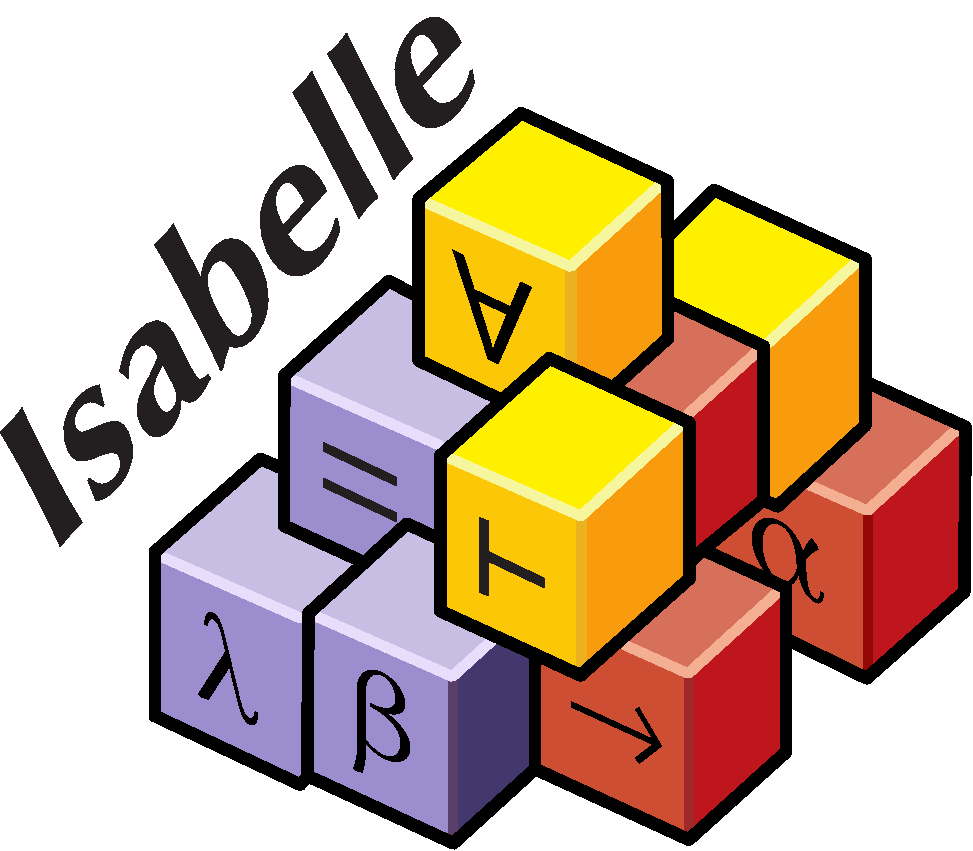
\includegraphics[width=.1\linewidth]{pics/isabelle.pdf}
  \end{tikzpicture}
  \end{center}
  
  \note[item]{Did the last slide say ``Copy \& Paste \textbf{without verification} into existing Docker rules''?}
  \begin{itemize}
  	\item So far
  	\begin{itemize}
  		\item Serializing new configurations
  	\end{itemize}
  	\item<2-> Missing
  	\begin{itemize}
  		\item Verify \texttt{iptables} filtering rules
  		\note<2->[item]{\emph{Bigger question}: understand arbitrary \emph{existing}, not just this docker}
  		\item Understanding \emph{arbitrary} \texttt{iptables} filtering rules
  		\note<2->[item]{\texttt{iptables} matching (security mechanism) is naturally more low level than policy}
  		\item \texttt{man iptables-extensions} over $200$ match options
  	\end{itemize}
  \end{itemize}
\end{frame}




\newcommand{\diffadd}[1]{\textcolor{TUMDarkGreen}{#1}}
\newcommand{\diffdel}[1]{\textcolor{TUMRed}{#1}}

\section{Understanding \texttt{iptables} with \fffuu{}}
\begin{frame}[fragile]

  \begin{columns}[t]
  \begin{column}{0.5\textwidth}
	\begin{itemize}
  		\item Input: \texttt{iptables-save}
  		\item Output:
  	\end{itemize}
  \begin{center}
  \begin{tikzpicture}
	%\node[align=center,text width=9.5em,cloud, draw,cloud puffs=10,cloud puff arc=120, aspect=2, inner sep=-3em,outer sep=0] (a) at (3,0) { $\{0.0.0.0 .. 9.255.255.255\} \cup \{11.0.0.0 .. 255.255.255.255\}$ }; %INET
	\node[align=center,text width=9.5em,cloud, draw,cloud puffs=10,cloud puff arc=120, aspect=2, inner sep=-3em,outer sep=0] (a) at (3,0) { \emph{INET} }; %INET
	\node (b) at (3,-2) { \emph{$\{10.0.0.4\}$} }; % WebApp
	\node (c) at (3,-4) { \emph{$\{10.0.0.3\}$} }; % DB
	\node (d) at (0,-3) { \emph{$\{10.0.0.2\}$} }; % Log
	\node (e) at (0,-1) { \emph{$\{10.0.0.1\}$} }; % WebFrnt
	\visible<1,2,3>{\node (f) at (2,-5) { \emph{\textcolor<3>{TUMRed}{$\{10.0.0.0\} \cup \{10.0.0.5 .. 10.255.255.255\}$}} };}% unused docker subnet mynet

	%\draw[myptr] (a) to[out=330,in=310,looseness=3] (a);
	\draw[myptr] (a) to[loop right] (a);
	\draw<1,2>[myptr] (a) to (b);
	\draw<1,2>[myptr] (a) to[bend left] (c);
	\draw<1,2>[myptr] (a) to (d);
	\draw<3>[myptr,TUMRed] (a) to[bend left] (c);
	\draw<3>[myptr,TUMRed] (a) to (d);
	\draw[myptr] (a) to (e);
	\draw<1,2>[myptr] (a) to[bend right] (f);
	\draw<3>[myptr,TUMRed] (a) to[bend right] (f);
	\draw[myptr] (b) to (a);
	\draw[myptr] (b) to[loop right] (b);
	\draw[myptr] (b) to (c);
	\draw[myptr] (b) to (d);
	\draw[myptr] (b) to (e);
	\draw<1,2>[myptr] (b) to[bend right] (f);
	\draw<3>[myptr,TUMRed] (b) to[bend right] (f);
	\draw[myptr] (c) to (b);
	\draw[myptr] (c) to[loop right] (c);
	\draw[myptr] (c) to (d);
	\draw[myptr] (d) to[loop below] (d);
	\draw[myptr] (e) to (b);
	\draw[myptr] (e) to (d);
	\draw[myptr] (e) to[loop above] (e);
	
	%draw over other arrow
	\draw<3>[myptr,TUMRed] (a) to (b);
	
	\draw[myptrdotted,orange] ($(e) + (3ex,1.5ex)$) to[bend left=15] (a);
	\visible<4->{\draw[myptrdotted,orange] (a) to[bend left=15] (b);}
	\end{tikzpicture}%
  \end{center}
  \note{Only \texttt{iptables-save}, so we only see ip addresses. Verification: Of course the copy\&paste step was unsound. We cannot simply combine low-level rules from the docker daemon with our custom rules. But we see: graphs similar, not that bad. 
  First: at the bottom, unused IP range from our docker subnet. Problem: INET can connect to anyone (interaction of our rules with docker-generated ones)! Works for arbitrary \texttt{iptables} filter tables, not just docker!
  Fun fact: ITval (competing tool for \texttt{iptables} analysis segfaults on this these rules.)
  %tested again with ITVAL-1.0 with my iptables-save Thu Sep 15 13:42:24 2016
  }
  
  \note<3->[item]{By the way, all connected to the same docker bridge, no spoofing protection. Also get this from \fffuu{}, not shown.}
  
  \note<3->[item]{removed unused docker subnet}
  \note<4->[item]{constrained Internet's access rights}
  
  \onslide<4,5>{} %force 5 slides	
  
  
  \end{column}
  \begin{column}{0.3\textwidth}
  \onslide<2->{
	\begin{itemize}
  		\item Recall the policy:
  	\end{itemize}
    \begin{center}
  	\resizebox{0.9\textwidth}{!}{%
    \begin{Large}
    \begin{tikzpicture}
        %note, different coordinates (tighter packed) than images with ipaddresses
	   	\node[align=center,text width=9.5em,cloud, draw,cloud puffs=10,cloud puff arc=120, aspect=2, inner sep=-3em,outer sep=0] (a) at (3,0) { \emph{INET} };
	   	\node (c) at (3,-2) { \emph{WebApp} };
	   	\node (d) at (3,-4) { \emph{DB} };
	   	\node (e) at (0,-3) { \emph{Log} };
	   	\node (b) at (0,-1) { \emph{WebFrnt} };
	   	
	   	\draw[myptr] (a) to[out=330,in=310,looseness=3] (a);
	   	\draw[myptr] (a) to (b);
	   	%\draw[myptr] (b) to (a);} %manually refined
	   	%manually refined by admin, reverify change with \topos{}
	   	\draw[myptr] (b) to[loop above] (b);
	   	\draw[myptr] (b) to (c);
	   	\draw[myptr] (b) to (e);
	   	\draw[myptr] (c) to (a);
	   	\draw[myptr] (c) to (b);
	   	\draw[myptr] (c) to[loop right] (c);
	   	\draw[myptr] (c) to (d);
	   	\draw[myptr] (c) to (e);
	   	\draw[myptr] (d) to (c);
	   	\draw[myptr] (d) to[loop right] (d);
	   	\draw[myptr] (d) to (e);
	   	\draw[myptr] (e) to[loop below] (e);
	   	
	   	\draw[myptrdotted,orange] (a) to[bend left=15] (c);
	   	\draw[myptrdotted,orange] ($(b) + (3ex,1.5ex)$) to[bend left=15] (a);
    \end{tikzpicture}
    \end{Large}}
    \end{center}
  }
  
  \onslide<4>{
	\begin{itemize}
  		\item Changing \texttt{iptables} rules
  	\end{itemize}
  \begin{tiny}
	\texttt{\diffdel{--A MYNET -i \dockerbr{} -s 10.0.0.4 ! -o \dockerbr{} -j ACCEPT}}\\
	\texttt{\diffdel{--A MYNET ! -i \dockerbr{} -o \dockerbr{} -d 10.0.0.1 -j ACCEPT}}\\
	\texttt{\diffadd{+-A MYNET -i \dockerbr{} -s 10.0.0.4 ! -o \dockerbr{} ! -d 10.0.0.0/8 -j ACCEPT}}\\
	\texttt{\diffadd{+-A MYNET ! -i \dockerbr{} ! -s 10.0.0.0/8 -o \dockerbr{} -d 10.0.0.1 -j ACCEPT}}\\
	\texttt{~-A MYNET -i \dockerbr{} -j DROP}\\
	\texttt{\diffadd{+-A MYNET -o \dockerbr{} -j DROP}}\\
	\texttt{\diffadd{+-A MYNET -s 10.0.0.0/8 -j DROP}}\\
	\texttt{\diffadd{+-A MYNET -d 10.0.0.0/8 -j DROP}}\\
	\end{tiny}
  }
  \end{column}
  \end{columns}
  
	\begin{tikzpicture}[overlay]
	\node (overviewcomponents) at ($(current page.south west)+(+11.2em,1em)$) {
	    \resizebox{0.4\textwidth}{!}{%
	 	\begin{tikzpicture}
		 \node [MyRoundedBox,fill=TUMIvony](sinvar) at (0,0) {\strut{}Security Requirements};
		 \node [MyDoubleArrow,fill=TUMIvony](arr1) at (sinvar.east) {};
		 \node [MyRoundedBox,fill=TUMIvony](policy) at (arr1.east) {\strut{}Security Policy};
		 \node [MySingleLeftArrow,fill=TUMYellow](arr2) at (policy.east) {};
		 \node [MyRoundedBox](mechanism) at (arr2.west) {\strut{}\texttt{iptables}};
		 \end{tikzpicture}
		 }
	};
	\end{tikzpicture}
\end{frame}

\section{Ultimately}
\begin{frame}
  \begin{center}
  \begin{tikzpicture}
  \node [MyRoundedBox](sinvar) at (0,0) {\strut{}Security Requirements};
  \node [MyDoubleArrow](arr1) at (sinvar.east) {};
  \node [MyRoundedBox](policy) at (arr1.east) {\strut{}Security Policies};
  \node [MyDoubleArrow](arr2) at (policy.east) {};
  \node [MyRoundedBox](mechanism) at (arr2.east) {\strut{}\texttt{iptables}};
  
  \node[anchor=south] at ($(arr1.south)+(1em,2em)$) {\resizebox{!}{10ex}{\yes}};
  \node[anchor=south] at ($(arr2.south)+(1em,2em)$) {\resizebox{!}{10ex}{\yes}};
  % 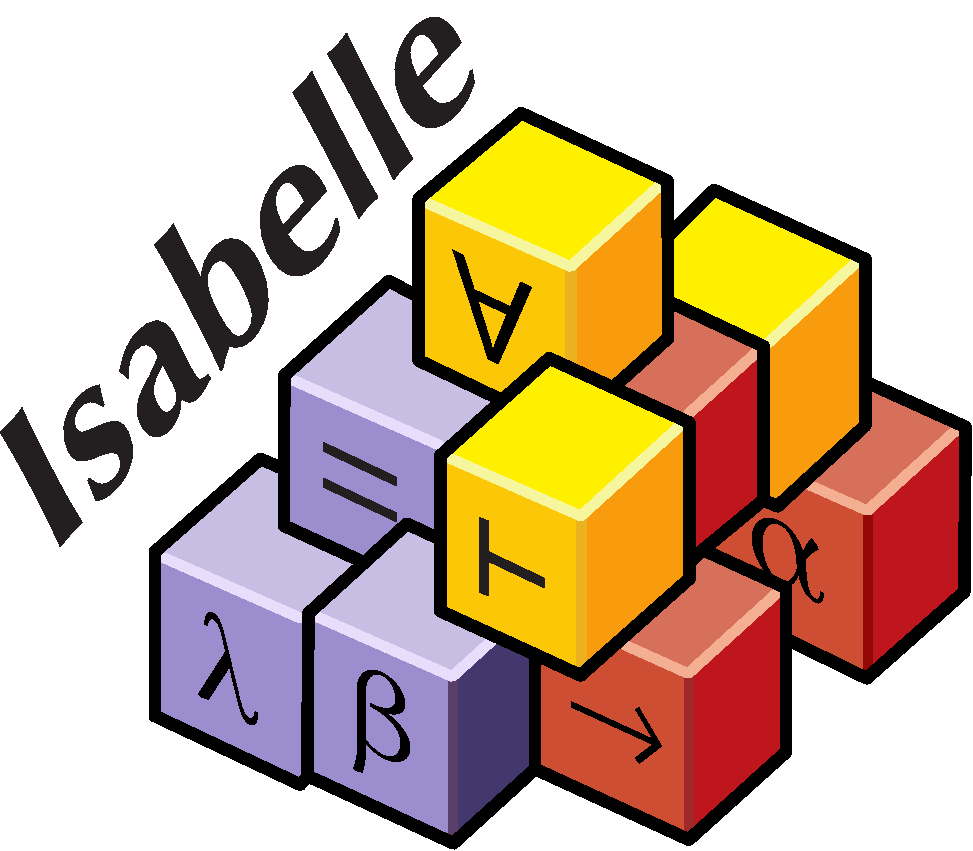
\includegraphics[width=.1\linewidth]{pics/isabelle.pdf}
  \end{tikzpicture}
  \end{center}
\end{frame}


\section{Related Work}

\begin{frame}
	%\frametitle{Leaving Nothing to be Desired\only<9->{: Related Work}}
	\tikzstyle{na} = [baseline=-.6ex]
	%
	\note[item]{Want: Tools \& languages to help us with these problems. What exactly do we want?}
	\note[item]{\yes{} yes}
	\note[item]{\wyes{} weaker yes, ``yes but \dots''}
	\note[item]{\no{} no}
	\begin{table}
	\begin{small}
		\begin{tabular}[0.99\linewidth]{ l  c  c  c  c  c  c  c}
			\toprule
			%Tool \textbackslash criterion
			                   & \tikz[na]\node(fsem){\parbox[t]{5em}{\centering Formal\\Semantics}};
			                   & \tikz[na]\node(fveri){\parbox[t]{5em}{\centering Formal\\Verification}};
			                   & \tikz[na]\node(hll){\parbox[t]{5em}{\centering High-Level\\Language}};  
			                   & \tikz[na]\node(vspec){\parbox[t]{5em}{\centering Built-In\\Verification}};
			                   & \tikz[na]\node(ct){\parbox[t]{5em}{\centering Connection\\Semantics}}; 
			                   & \tikz[na]\node(legsup){\parbox[t]{5em}{\centering Legacy\\Support}}; 
			                   & \tikz[na]\node(llacc){\parbox[t]{5em}{\centering Low Level\\Access}}; 
			\onslide<9->{\\\midrule}%
	\onslide<10->{NetCore            & \yes     & \yes      & \no  & \wyes     & \no  & \no     & \no       }\\
	\note<10>{NetCore: stateless SDN forwarding language. Formal semantics of \textbf{language} and \textbf{OpenFlow controller} (hw, security mechanism). Coq. First machine verified SDN controller.}%
	\note<10>{Also: There are means to verify a NetCore program.}%
	%
	\onslide<10->{NetKAT family      & \yes     & \wyes     & \no  & \wyes     & \no  & \no     & \no       }\\
	\note<10>{NetKAT: Successor to NetCore (more cool features, not everything formally verified in theorem prover). Nice built-in verification capabilities: Automatically check equivalence of two NetKAT statements}%
	%
	\onslide<11->{VALID              & \wyes    & \no       & \yes & \no       & \no  & \no     & \no       }\\
	\note<11>{VALID: high-level language to express security requirements. Formally defined in AVISPA (validation toolset not theorem prover (definitions not total, strictly mathematically well-typed, \dots), we complain on a very high level here). Can verify that a given network topology conforms to specified high-level goals, but cannot serialize goals to a network topology nor give feedback about the meaning of the specified goals.}%
	%
	\onslide<11->{Zhao et al.        & \no      & \no       & \yes & \no       & \no  & \no     & \no       }\\
	\note<11>{Zhao et al: policy refinement framework for networks. Short: translate high level requirements to network configurations.}%
	%
	\onslide<12->{Flowlog \& co      & \no      & \no       & \no  & \yes      & \yes & \yes    & \no       }\\
	\note<12>{Flowlog: event-driven language with a syntax similar to SQL. ct! especially designed with built-in verification and analysis in mind: You write a flowlog program and get automated(!!) feedback about it. Or semantical diff of two programs, ... Legacy: Translate huge fraction of Cisco IOS router configs to flowlog.}%
	%
	\onslide<13->{Mignis             & \wyes    & \wyes     & \no  & \no       & \yes & \no     & \wyes     }
	\note<13>{Mignis: formal semantics (on paper) of \texttt{iptables}. Translate their policy language to \texttt{iptables} (proof on paper). Conntrack, NAT, ... support. Allow users to add custom low-level \texttt{iptables} match conditions into their language as string. Not sound for certain match extensions, no method to figure out whether my string introduces soundness issues. }%
	%\onslide<7->{\midrule}
	%		\midrule
	\onslide<14->{\\\midrule}%
	\note<15->{Everything formalized and proven in Isabelle/HOL, thy in AFP. \topos{} high-level easy-to-use language which exposes few formalism to admin. Gives visual feedback about your requirement spec. Compiles to network (iptables, openflow), considers state. Admin can refine intermediate results and re-verify. \fffuu{} understands you legacy iptables config, makes it available to \topos{}. }%
	\onslide<15->{\topos{} + \fffuu{}& \tikz[na]\node(myyes1){\yes}; & \tikz[na]\node(myyes2){\yes}; & \yes & \yes      & \yes & \yes    & \yes      }
			\onslide<15->{\\\bottomrule}%
		\end{tabular}%
	\end{small}
	\end{table}
	
	\begin{tikzpicture}[overlay]
		\node<2>[anchor=north west] (fsemlabel) at ($(current page.west)+(5em,0)$) {\begin{varwidth}{\linewidth}Formal Semantics
			\begin{itemize}
				\item Management language
				\item Target security mechanism
				\item Type checked by theorem prover
			\end{itemize}	
		\end{varwidth}	
		};
	    \path[myptr]<2> ($(fsemlabel.north west)+(3em,0)$) edge (fsem.south); %
	    
	    
		\node<3>[anchor=north west] (fverilabel) at ($(current page.west)+(5em,0)$) {\begin{varwidth}{\linewidth}Formal Verification
			\begin{itemize}
				\item Compilation/translation verified: Language $\rightarrow$ Mechanism
				\item Proof machine-checked
			\end{itemize}	
		\end{varwidth}	
		};
	    \path[myptr]<3> ($(fverilabel.north west)+(3em,0)$) edge ($(fveri.south)+(-1ex,0)$); %
	    
	    
		\node<4>[anchor=north west] (hlllabel) at ($(current page.west)+(5em,0)$) {\begin{varwidth}{\linewidth}High-Level Language
			\begin{itemize}
				\item Security requirements, not policy
			\end{itemize}	
		\end{varwidth}	
		};
	    \path[myptr]<4> ($(hlllabel.north west)+(3em,0)$) edge ($(hll.south west)+(0,.5ex)$); %
	    
	    
		\node<5>[anchor=north west] (vspeclabel) at ($(current page.west)+(5em,0)$) {\begin{varwidth}{\linewidth}Built-In Verification
			\begin{itemize}
				\item Of the \textbf{specification}
				\item Feedback
				\item Automated
			\end{itemize}	
		\end{varwidth}	
		};
	    \path[myptr]<5> ($(vspeclabel.north west)+(3em,0)$) edge ($(vspec.south west)+(0,.8ex)$); %
	    
	    
		\node<6>[anchor=north west] (ctlabel) at ($(current page.west)+(5em,0)$) {\begin{varwidth}{\linewidth}Stateful Connection Semantics
			\begin{itemize}
				\item \texttt{conntrack}
				\item Connection level vs.\ network level
				\item ``I can connect to the Internet, but not the other way round''
			\end{itemize}	
		\end{varwidth}	
		};
	    \path[myptr]<6> ($(ctlabel.north west)+(3em,0)$) edge ($(ct.south west)+(1ex,1ex)$); %
	    
	    
		\node<7>[anchor=north west] (legsuplabel) at ($(current page.west)+(5em,0)$) {\begin{varwidth}{\linewidth}Legacy Support
			\begin{itemize}
				\item Read \texttt{iptables}, Cisco, \ldots and make available to high-level abstraction
			\end{itemize}	
		\end{varwidth}	
		};
	    \path[myptr]<7> ($(legsuplabel.north west)+(3em,0)$) edge ($(legsup.south west)+(1ex,1ex)$); %
	    
	    
	    
		\node<8>[anchor=north west] (llacclabel) at ($(current page.west)+(5em,0)$) {\begin{varwidth}{\linewidth}Low Level Access
			\begin{itemize}
				\item Administrator may tune low-level configuration
				\item Soundness check
			\end{itemize}	
		\end{varwidth}	
		};
	    \path[myptr]<8> ($(llacclabel.north west)+(3em,0)$) edge ($(llacc.south west)+(1ex,1ex)$); %
	    
	    
	    \node<16->[anchor=south west] (isabelle) at ($(current page.south west)+(7em,.1em)$) {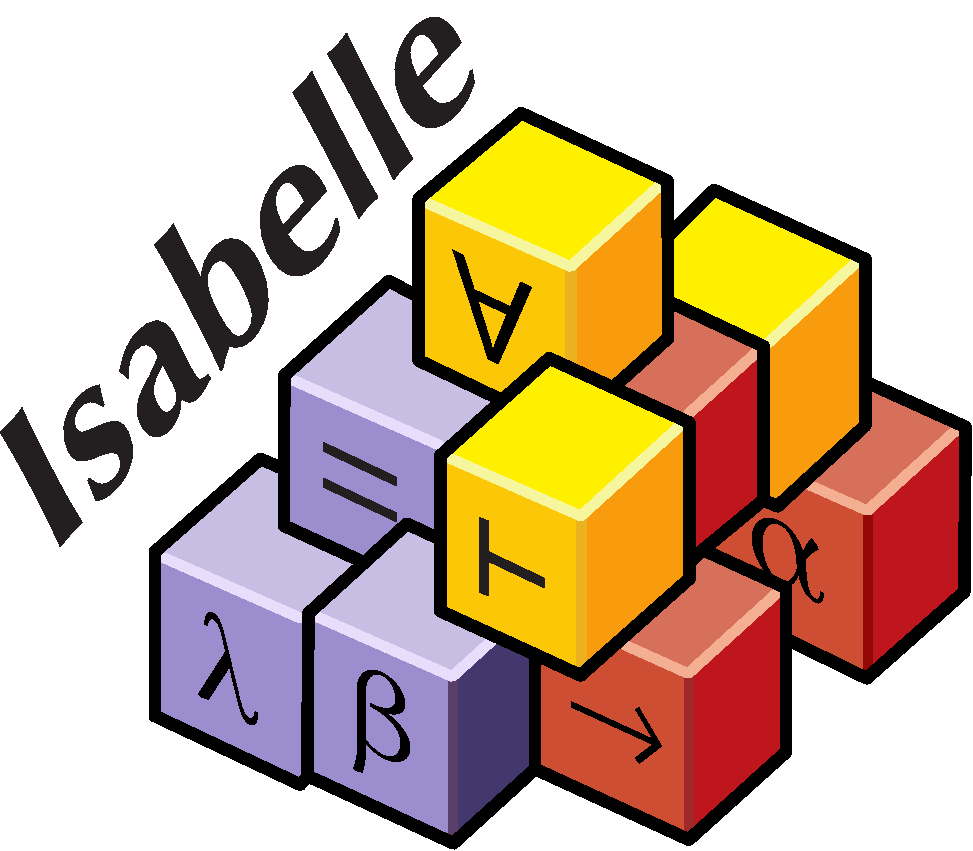
\includegraphics[width=.2\linewidth]{pics/isabelle.pdf}};
	    \path[myptr]<16-> ($(isabelle.north)+(1em,-1em)$) edge (myyes1); %
	    \path[myptr]<16-> ($(isabelle.north)+(1em,-1em)$) edge (myyes2); %
	\end{tikzpicture}
\end{frame}




\section{Conclusion}
\begin{frame}

  \begin{center}
  %\resizebox{0.99\textwidth}{!}{%
  \begin{tikzpicture}
  \node [MyRoundedBox](sinvar) at (0,0) {\strut{}Security Requirements};
  \node [MyDoubleArrow](arr1) at (sinvar.east) {};
  \node [MyRoundedBox](policy) at (arr1.east) {\strut{}Security Policies};
  \node [MyDoubleArrow](arr2) at (policy.east) {};
  \node [MyRoundedBox](mechanism) at (arr2.east) {\strut{}\texttt{iptables}};
 
  \path[draw,myptr,shorten >=0.5cm,shorten <=0.5cm] 
  (sinvar) to[bend left]    node[anchor=south, yshift=1ex] {\topos{} Policy Construction} (policy);

  \path[draw,myptr,shorten >=0.5cm,shorten <=0.5cm] 
  (policy) to[bend left]    node[anchor=south, yshift=1ex] {\topos{} Serialize} (mechanism);

  \path[draw,myptr,shorten >=0.5cm,shorten <=0.5cm] 
  (mechanism) to[bend left]    node[anchor=north, yshift=-1ex] {\fffuu{} Service Matrices} (policy);

  \path[draw,dashed,myptr,shorten >=0.5cm,shorten <=0.5cm] 
  (policy) to[bend left]    node[anchor=north, yshift=-1ex] {\topos{} Verification} (sinvar);
  \end{tikzpicture}%
  %}
  \end{center}
  
  
	\begin{itemize}
  		\item First, fully machine-verified tools for bridging the above gaps \emph{in both directions}
  		\item Evaluated on
  		\begin{itemize}
  			\item Cabin data network
  			\item Android Measurement System
  			\item Largest collection of public \texttt{iptables} dumps
  				\note{which we collected and published}
  		\end{itemize}
  		\item Published in
  		\begin{itemize}
  			\item AFP (x6), FM, FORTE (x2), IFIP NETWORKING, CNSM, CNSM Workshop, ESSS
  		\end{itemize}
  	\end{itemize}
\end{frame}

%%%%%%%%%%%%%%%%%%%%%%%%%% backup slides %%%%%%%%%%%%%%%%%%%%%%%%%

\section{Backup}
\begin{frame}
	\begin{center}
	\begin{Large}
	Backup Slides
	\end{Large}
	\end{center}
\end{frame}


%new publications: FORTE!
\section{Publications (AFP)}
\begin{frame}
	\begin{tikzpicture}[overlay]
	    \node[anchor=north] (isabelle) at ($(current page.north east)+(-8em,-3em)$) {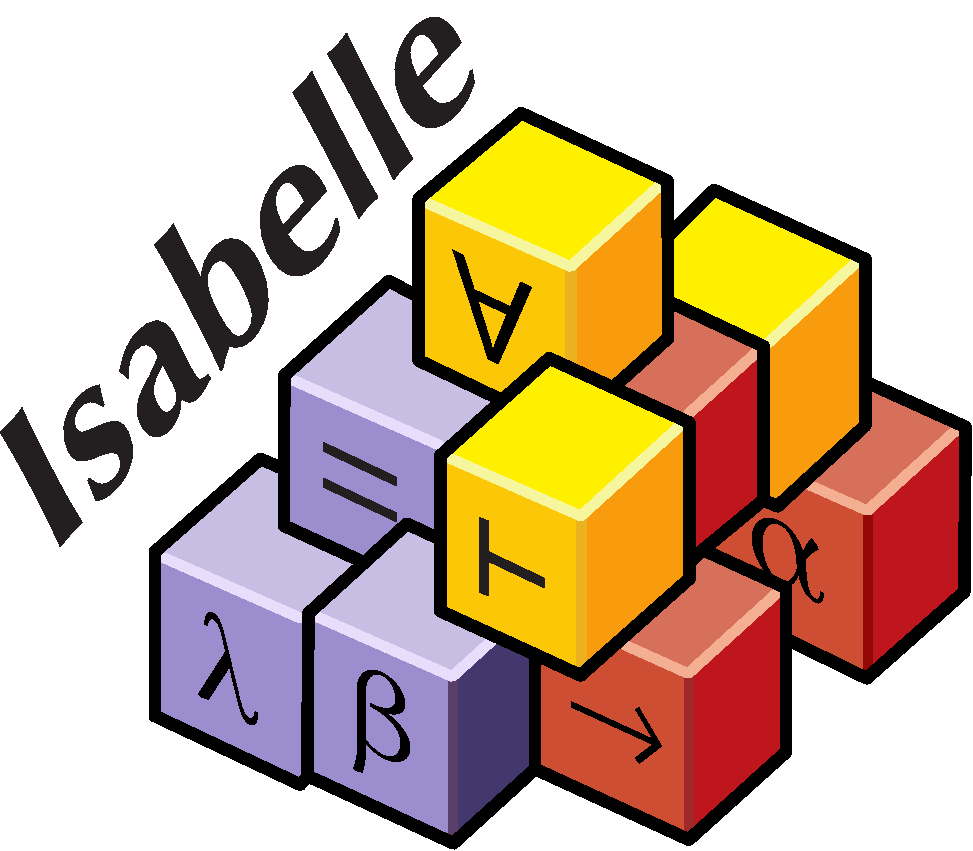
\includegraphics[width=.1\linewidth]{pics/isabelle.pdf}};
	\end{tikzpicture}
% fix: getting linebreaks before the location but not the title
% http://latex.org/forum/viewtopic.php?t=3215
\setbeamertemplate{bibliography entry title}{}
\setbeamertemplate{bibliography entry location}{}
\setbeamertemplate{bibliography entry note}{}
	\begin{itemize}
    	\footnotesize
    	\setlength{\itemsep}{0pt}
		\item \bibentry{LOFT-AFP}
		\item \bibentry{Iptables_Semantics-AFP}
		\item \bibentry{Routing-AFP}
		\item \bibentry{Simple_Firewall-AFP}
		\item \bibentry{IP_Addresses-AFP}
		\item \bibentry{Network_Security_Policy_Verification-AFP}
	\end{itemize}
\end{frame}

\section{Publications}
\begin{frame}[allowframebreaks]
% fix: getting linebreaks before the location but not the title
% http://latex.org/forum/viewtopic.php?t=3215
\setbeamertemplate{bibliography entry title}{}
\setbeamertemplate{bibliography entry location}{}
\setbeamertemplate{bibliography entry note}{}
%itemize setup
	%\topos{}\vspace{-\topsep}
	\begin{itemize}
    	\footnotesize
    	\setlength{\itemsep}{0pt}
		\item \bibentry{maltitz2016forte}
		\item \bibentry{maltitz2016fmpriv}
		\item \bibentry{diekmann2015topos}
		\item \bibentry{diekmann2014forte}
		\item \bibentry{diekmann2014EPTCS}
	%\end{itemize}
	%
	%\fffuu{}
	%\begin{itemize}
    %	\footnotesize
    %	\setlength{\itemsep}{0pt}
		\item \bibentry{diekmann2016networking}
		\item \bibentry{diekmann2015cnsm}
		\item \bibentry{diekmann2015fm}
	\end{itemize}
	\note[item]{New: Forte 2017}
	\note[item]{To appear soon: Naming Linux Network Interfaces in Poc||GTFO16}
	\note[item]{pending: 2 Journal submissions}
\end{frame}

%\section{Logo of \fffuu{}}
%\begin{frame}
%	\begin{center}
%	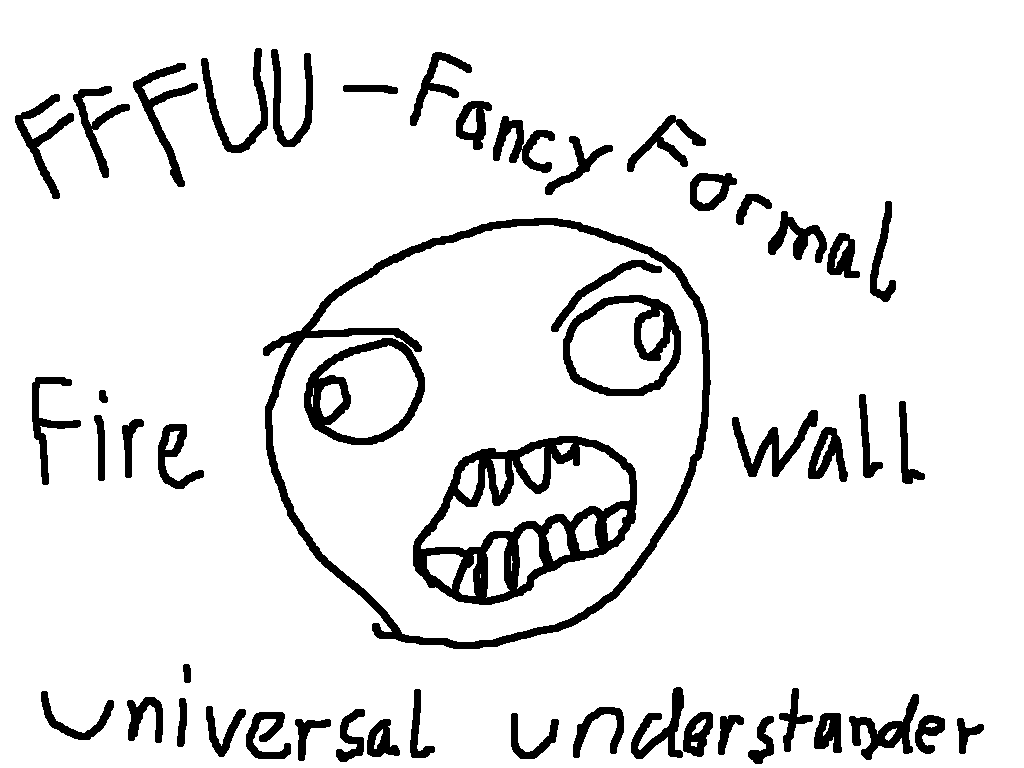
\includegraphics[width=.8\linewidth]{pics/fffuu.png}
%	\end{center}
%\end{frame}



\section{Central Theorem of \fffuu{}}
\begin{frame}
%	assumes agree:"matcher_agree_on_exact_matches γ common_matcher"
%	  and     simple: "simple_ruleset rs"
%	  and     new: "newpkt p"             
%	  and     matrix: "(V,E) = access_matrix ⦇pc_iiface = p_iiface p, pc_oiface = p_oiface p, pc_proto = p_proto p, pc_sport = p_sport p, pc_dport = p_dport p⦈ (to_simple_firewall (preprocess rs))"
%	  and     accept: "Γ,γ,p⊢ ⟨rs, Undecided⟩ ⇒ Decision FinalAllow"
%	  shows "∃s_repr d_repr s_range d_range. (s_repr, d_repr) ∈ set E ∧
%	              (map_of V) s_repr = Some s_range ∧ (p_src p) ∈ wordinterval_to_set s_range ∧
%	              (map_of V) d_repr = Some d_range ∧ (p_dst p) ∈ wordinterval_to_set d_range"
	Assumes	
	\begin{itemize}
		\item Unfolded $\free{\mvar{rs}}$ for $\free{\Gamma}$
		\item $\free{\mvar{p}}$ is \texttt{NEW}% and has \texttt{SYN} set (if TCP)
		\item $\bigstep{\free{\mvar{rs}}}{\undecided}{\allow}$
		\item Let $(\free{V}, \free{E}) = \mfun{matrix}\ (\mdef{iifce}\ \free{p}, \mdef{oifce}\ \free{p}, \mdef{prot}\ \free{p}, \mdef{sport}\ \free{p}, \mdef{dport}\ \free{p})\ (\mfun{simplify}\ \free{\mvar{rs}})$
	\end{itemize}
	Shows%
	\begin{center}%
		\vskip-3ex%
	    \begin{IEEEeqnarray*}{l}
		\exists \bound{\mvar{s}_\text{repr}}\ \bound{\mvar{d}_\text{repr}}\ \bound{\mvar{s}_\text{range}}\ \bound{\mvar{d}_\text{range}}.\ \ (\bound{\mvar{s}_\text{repr}}, \bound{\mvar{d}_\text{repr}}) \in  \mdef{set}\ \free{\mvar{E}} \  \wedge  \\
		\qquad (\mfun{map\_of}\ \free{\mvar{V}})\ \bound{\mvar{s}_\text{repr}} = \mdef{Some}\ \bound{\mvar{s}_\text{range}} \ \wedge \ (\mdef{src}\ \free{\mvar{p}}) \in \bound{\mvar{s}_\text{range}} \ \wedge \\
		\qquad (\mfun{map\_of}\ \free{\mvar{V}})\ \bound{\mvar{d}_\text{repr}} = \mdef{Some}\ \bound{\mvar{d}_\text{range}} \ \wedge \ (\mdef{dst}\ \free{\mvar{p}}) \in \bound{\mvar{d}_\text{range}}
		\end{IEEEeqnarray*}
	\end{center}
	\medskip
	Reads: If the firewall accepts a packet, we can look up source and destination IP in the graph.
	
	\begin{itemize}
		\item Unfolding may fail (it is successful if the kernel accepts it and it has no `strange' actions)
		\item We can ignore interfaces if we have spoofing protection
	\end{itemize}
\end{frame}


\subsection{Abstraction Layers}
\begin{frame}
	\begin{center}
	\resizebox{0.45\linewidth}{!}{%
	\Large
	\begin{tikzpicture}
	\node[text width=0.3\linewidth, align=center] (iheardyoulikerecursion) at (0,1.5) {
				\resizebox{.99\linewidth}{!}{
					\scalebox{2}{\Huge{$P($}}\Large\begin{tikzpicture} [baseline=-3ex]
					\node[anchor=south] (bi) at (0,0) {Bob};
					\node[anchor=east] (ai) at (-.9,-.6) {Alice};
					\node[anchor=west] (ci) at (+.9,-.6) {Carl};
					
					\draw[myptr] (ai) to (bi);
					\draw[myptr] (bi) to (ci);
					\draw[myptr,shorten >=1ex] (ci) to (ai.east); %yolo irgendwie geht der arrow zu weit
					\end{tikzpicture}\scalebox{2}{\Huge{$)$}}%
				}
			};
	
	\def\sbordery{+.9}
	\draw [thick,dashed] (-3,\sbordery)--(3,\sbordery);
	\node[anchor=south west, align=left, text width=6em] at (3.,\sbordery) {Security\\Invariants};
	
	
	\node[anchor=south] (b) at (0,0) {Bob};
	\node[anchor=east] (a) at (-.9,-.6) {Alice};
	\node[anchor=west] (c) at (+.9,-.6) {Carl};
	
	\draw[myptr,shorten >=-1ex,shorten <=-1ex] (a) to (b);
	\draw[myptr,shorten >=-1ex,shorten <=-1ex] (b) to (c);
	\draw[myptr] (c) to (a);
	
	\def\abordery{-1.3}
	\draw [thick,dashed] (-3,\abordery)--(3,\abordery);
	\node[anchor=south west, align=left, text width=6em] at (3.,\abordery) {Access\\Control\\Abstraction};
	
	\node[server,label=below:Alice] (ra) at (-2.5,-3.5) {};
	\node[server,label=below:Bob] (rb) at (0,-2) {};
	%\node[server,label={[xshift=.5ex, yshift=-1ex]left:Carl}] (rc) at (2.,-4.5) {};
	\node[server,label=below:Carl] (rc) at (2.,-4.5) {};
	\node[switch] (aux1) at (-1.2,-3.4) {};
	\node[router] (aux2) at (1.5,-3.2) {};
	\node[router] (aux3) at (.3,-4.3) {};
	
	\draw[thick] (ra) to (aux1);
	\draw[thick] (rb) to (aux2);
	%\draw[thick] (aux) to (rc);
	\draw[thick] (rc) to (aux2);
	\draw[thick] (aux1) to (aux2);
	\draw[thick] (aux2) to (aux3);
	\draw[thick] (aux1) to (aux3);
	
	
	\draw [dotted,thick] (a)--(-2.5,-1)--(ra);
	\draw [dotted,thick] (b)--(rb);
	\draw [dotted,thick] (c)--($(2.,-1)+(1ex,0)$)--($(rc.north)+(1ex,0)$);
	
	\def\ibordery{-5.5}
	\draw [thick,dashed] (-3,\ibordery)--(3,\ibordery);
	\node[anchor=south west, align=left, text width=6em] at (3.,\ibordery) {Interface\\Abstraction};
	
	\node[anchor=north] (l1) at (-2.,-5.8) {
\includegraphics[height=2.5em]{pics/puf.pdf}};
	\draw [dotted,thick] (aux1)--(l1);
	
	
	\node[anchor=north, align=center, text width=5em] (l3) at (0,-5.9) {\small{\parbox[c]{5em}{\centering Commercial Product}}};
	\draw [dotted,thick] (aux3)--(l3);
	
	
	\node[anchor=north] (l2) at (2.,-5.8) {
\includegraphics[height=2.5em]{pics/tux.pdf}};
	\draw [dotted,thick] ($(aux2.south)+(-1ex,0)$)--($(1.5,-5.3)+(-1ex,0)$)--(l2);
	
	\def\bbordery{-7}
	\node[anchor=south west, align=left, text width=6em] at (3.,\bbordery) {Box\\Semantics};
	
	\end{tikzpicture}}%
	\end{center}
\end{frame}


\subsection{Related Work}
\begin{frame}
	
	\newcommand{\AccessControlVerifySinvars}[0]{VALID~\cite{bleikertz2011VALID}; \topos{}\phantom{;}}
	\newcommand{\SinvarsToAccessControl}[0]{Zhao~\etal\cite{zhao2011policyremanet}; \mbox{\topos{} step \emph{B}}}
	
	\newcommand{\boxSemanticsToAccessControlAbstraction}[0]{Fireman~\cite{fireman2006}; ITVal~\cite{marmorstein2006firewall}; \mbox{\fffuu{}\phantom{;}}}
	\newcommand{\InterfaceAbstractionToAccessControl}[0]{Fireman~\cite{fireman2006}; HSA~\cite{kazemian2012HSA}; Anteater~\cite{Mai2011anteater}; \mbox{ConfigChecker}~\cite{alshaer2009configchecker}; VeriFlow~\cite{khurshid2013veriflow}}
	\newcommand{\InterfaceAbstractionMAPSAccessControl}[0]{Xie~\cite{xie2005static}; Lopes~\cite{lopes2013msrnetworkverificationprogram}}
	\newcommand{\BoxSemanticsMAPSInterfaceAbstraction}[0]{HSA~\cite{kazemian2012HSA}; Anteater~\cite{Mai2011anteater}; Config\-Checker~\cite{alshaer2009configchecker}}
	\newcommand{\AccessControlToInterfaceAbstraction}[0]{one big\phantom{;} switch~\cite{monsanto2013composingonebigswitch}; Firmato~\cite{bartal1999firmato}; FLIP~\cite{ZhangAlShaer2007flip}; \mbox{FortNOX}~\cite{Porras2012FortNOX}; Merlin~\cite{soule2014merlin}; Kinetic~\cite{kinetic2015}; \mbox{PBM~\cite{dinesh2002policybased}\phantom{;}}}
	\newcommand{\AccessControlToBoxSemantics}[0]{Firmato~\cite{bartal1999firmato}; FLIP~\cite{ZhangAlShaer2007flip}; NetKAT~\cite{icfp2015smolkanetkatcompiler};\newline{}Mignis~\cite{mignis2014};\newline Or-BAC~\cite{orbacnetwork04}; \topos{} step \emph{C}+\emph{D}}
	\newcommand{\InterfaceAbstractionToBoxSemantics}[0]{RCP~\cite{Caesar2005rcp}; \mbox{OpenFlow}~\cite{mckeown2008openflow}; Merlin~\cite{soule2014merlin}; \mbox{optimized one}\phantom{;} \mbox{big switch}~\cite{Kang2013onebigswitchabstraction}; NetKAT~\cite{icfp2015smolkanetkatcompiler}; VeriFlow~\cite{khurshid2013veriflow}; FML~\cite{hinrichs2009practical}\phantom{;}}
	\newcommand{\BoxSemantics}[0]{\mbox{Iptables Semantics}~\cite{diekmann2015fm}}

	\begin{center}
    \resizebox{!}{0.99\textheight}{%
 	\begin{tikzpicture}
	 \node [MyRoundedBox, text width=13em](abs1) at (0,0) {Security Invariants};
	 \node [MyRoundedBox, text width=13em](abs2) at (0,-2) {Access Control Abstraction};
	 \node [MyRoundedBox, text width=13em](abs3) at (0,-6) {Interface Abstraction};
	 \node [MyRoundedBox, text width=13em](abs4) at (0,-10) {Box Semantics};
	 
	 \draw [thick,-to,->] ($(abs1.south) + (+3em,0)$)--($(abs2.north) + (+3em,0)$);
	 \node [anchor=west, align=left, text width=12em] at ($(abs1)!0.5!(abs2) + (+3.2em,0)$) {\SinvarsToAccessControl};
	 
	 \draw [thick,-to,dashed,->] ($(abs2.north) + (-3em,0)$)--($(abs1.south) + (-3em,0)$);
	 \node [anchor=east, align=right, text width=7em] at ($(abs1)!0.5!(abs2) + (-3.2em,0)$) {\AccessControlVerifySinvars};
	 
	 \draw [thick,-to,->] ($(abs2.east) + (0,-0.8ex)$)--($(abs2.east) + (+6em,-0.8ex)$)--($(abs3.east) + (+6em,+0.8ex)$)--($(abs3.east) + (0,+0.8ex)$);
	 \node [anchor=east, align=right, text width=7em] at ($(abs2)!0.5!(abs3) + (+12.8em,0)$) {\AccessControlToInterfaceAbstraction};
	 
	 
	 \draw [thick,-to,dotted,->] ($(abs3.north) + (-2em,0)$)--($(abs2.south) + (-2em,0)$);
	 \node [anchor=west, align=left, text width=7em] at ($(abs3)!0.5!(abs2) + (-1.8em,0)$) {\InterfaceAbstractionMAPSAccessControl};
	 
	 \draw [thick,-to,->] ($(abs3.east) + (0,-0.8ex)$)--($(abs3.east) + (+6em,-0.8ex)$)--($(abs4.east) + (+6em,+0.8ex)$)--($(abs4.east) + (0,+0.8ex)$);
	 \node [anchor=east, align=right, text width=7em] at ($(abs3)!0.5!(abs4) + (+12.8em,0)$) {\InterfaceAbstractionToBoxSemantics};
	 \draw [thick,-to,->] ($(abs2.east) + (0,+0.8ex)$)--($(abs2.east) + (+6.8em,+0.8ex)$)--($(abs4.east) + (+6.8em,-0.8ex)$)--($(abs4.east) + (0,-0.8ex)$);
	 \node [anchor=west, align=left, text width=8em] at ($(abs2)!0.5!(abs4) + (+14.0em,0)$) {\AccessControlToBoxSemantics};


	 \draw [thick,-to,dotted,->] ($(abs4.north) + (-2em,0)$)--($(abs3.south) + (-2em,0)$);
	 \node [anchor=west, align=left, text width=7em] at ($(abs4)!0.5!(abs3) + (-1.8em,0)$) {\BoxSemanticsMAPSInterfaceAbstraction};	 
	 
	 \draw [thick,-to,dashed,->] ($(abs3.west) + (0,+0.8ex)$)--($(abs3.west) + (-6em,+0.8ex)$)--($(abs2.west) + (-6em,-0.8ex)$)--($(abs2.west) + (0,-0.8ex)$);
	 \node [anchor=west, align=left, text width=9em] at ($(abs2)!0.5!(abs3) + (-12.9em,0)$) {\InterfaceAbstractionToAccessControl};
	 
	 %\draw [thick,-to,->] ($(abs4.west) + (0,+0.8ex)$)--($(abs4.west) + (-7em,+0.8ex)$)--($(abs3.west) + (-7em,-0.8ex)$)--($(abs3.west) + (0,-0.8ex)$);
	 \draw [thick,-to,dashed,->] ($(abs4.west) + (0,-0.8ex)$)--($(abs4.west) + (-0.8em,-0.8ex)$)--($(abs4.west) + (-0.8em,+3)$)--($(abs4.west) + (-6.8em,+3)$)--($(abs2.west) + (-6.8em,+0.8ex)$)--($(abs2.west) + (0,+0.8ex)$);
	 \node [anchor=east, align=right, text width=6em] at ($(abs2)!0.4!(abs4) + (-14.0em,0)$) {\boxSemanticsToAccessControlAbstraction};
	 
	 
	 \draw [thick,-to,->] ($(abs4.south) + (-3em,0)$)--($(abs4.south) + (-3em,-3ex)$)--($(abs4.south) + (+3em,+-3ex)$)--($(abs4.south) + (+3em,0)$);
	 \node [anchor=north, align=center, text width=10em] at ($(abs4.south)+ (0,-3ex)$) {\BoxSemantics};
	 
	 
	 \draw[thick,-to,->] (-3,-8) to node[above,sloped]{translates} (-3,-10);
	 \draw[thick,-to,dotted,<-] (-2.25,-8) to node[above,sloped]{maps} (-2.25,-10);
	 \draw[thick,-to,dashed,<-] (-1.5,-8) to node[above,sloped]{verifies} (-1.5,-10);
	 \end{tikzpicture}
	}
	\end{center}
\end{frame}


% Include markdown source from ./pandoc
%\input{pandoc/example}

% Comment out if you do not want a bibliography
\section{Bibliography}
\begin{frame}[allowframebreaks]
    \bibliographystyle{abbrv}
    \setbeamertemplate{bibliography item}[text]
    \footnotesize
    \bibliography{literature}
\end{frame}

\end{document}

